\documentclass[11pt]{article}
\usepackage[a4paper,margin=2.5cm]{geometry}
\usepackage{amsmath,amssymb,amsthm,graphicx,booktabs,xcolor}
\usepackage[colorlinks=true,linkcolor=blue!60!black,citecolor=blue!60!black,urlcolor=blue!60!black]{hyperref}
\usepackage{xurl}
\hypersetup{pdftitle={How Much Infinity Does Physics Need?},pdfauthor={Ruqing Chen}}
\setlength{\emergencystretch}{3em}
\graphicspath{{../figures/}{figures/}{./}}

\newtheorem{theorem}{Theorem}
\newtheorem{proposition}{Proposition}[section]
\newtheorem{corollary}{Corollary}[section]
\newtheorem{lemma}{Lemma}[section]
\theoremstyle{definition}\newtheorem{definition}{Definition}[section]
\theoremstyle{remark}\newtheorem*{remark}{Remark}

\newcommand{\RCA}{\mathsf{RCA}_0}
\newcommand{\WKL}{\mathsf{WKL}_0}
\newcommand{\ACA}{\mathsf{ACA}_0}
\newcommand{\PA}{\mathsf{PA}}
\newcommand{\REC}{\mathrm{REC}}
\newcommand{\paperdoi}{10.5281/zenodo.23212848}

\title{How Much Infinity Does Physics Need?\\
Reverse Mathematics of Physical Limits\\ and the Empirical Boundary}
\author{Ruqing Chen\\[2pt]
\small GUT Geoservice Inc., Montreal, Quebec, Canada\\
\small \href{mailto:ruqing@hotmail.com}{\texttt{ruqing@hotmail.com}}}
\date{\small DOI: \href{https://doi.org/\paperdoi}{\paperdoi}}

\begin{document}
\maketitle

\begin{abstract}
Infinite limits are everywhere in physics: thermodynamic limits, infrared limits of renormalisation-group flows,
fractal dimensions, and limit sets. We ask how much set existence such limits require, in the sense of reverse
mathematics, and we compare the answer with what finite experiments can certify.

We prove four equivalences over $\RCA$. Each of the following is equivalent to arithmetical comprehension $\ACA$:
Fekete's lemma for subadditive sequences, which underlies the existence of thermodynamic limits; the existence of the
infrared limit of every bounded monotone $c$-function; the existence of the scaling exponent of every Cantor construction
with nondecreasing dimension parameters; and the existence of the set of indices whose computable fractal limit sets
are connected. At the level of individual quantities, a limit whose convergence has a computable modulus that $\RCA$
can verify is provably existent in $\RCA$. A limit that is not a computable real is not, because the $\omega$-model $\REC$
of computable sets contains no real equal to it.

We classify the limits used in a series of nine papers accordingly. The quantities for which explicit certification
budgets were found come with explicit moduli and are provable in $\RCA$. This includes the Ising free energy, whose
finite-size error is $0.639913/L^2$ at criticality, matching the Ising CFT torus amplitude
$\ln[(\theta_2+\theta_3+\theta_4)/2\eta](i)=0.639912$. It also includes the critical-cluster mass of the diamond lattice, with
geometric modulus $\Lambda_2/\Lambda_1=0.3553$, and the embezzlement asymptotics, with error $O(1/(n\ln n))$. The quantities
that need $\ACA$ are exactly those defined by limits without computable modulus: a fractal dimension equal to a
function of Chaitin's $\Omega$, the connectivity of limit sets, and the finite-dimensional values of nonlocal games. These
are precisely the quantities shown elsewhere to be empirically inaccessible. Since $\ACA$ is conservative over Peano
arithmetic, the infinity that these physical limits require is real but logically mild. The only result in the series
whose logical strength is unknown is the classification of injective von Neumann algebras.
\end{abstract}

\tableofcontents

%=====================================================================
\section{Introduction}
\label{sec:intro}

Reverse mathematics asks which set-existence axioms are needed to prove a theorem of ordinary
mathematics~\cite{Friedman,Simpson}. Most theorems of analysis turn out to be provable in, or equivalent over a weak base
theory to, one of a few subsystems of second-order arithmetic. Feferman argued that the mathematics actually used in
the sciences can be formalised in a system conservative over Peano arithmetic~\cite{Feferman}. Physics thus needs
only a little of the infinite.

This paper makes that statement precise for the limits that occur in physics, and relates it to a different question:
which limits can be certified by finite experiments? In a series of papers we found sharp answers to the second
question. Fractal dimensions can be uncomputable~\cite{Chen2026_chaitin}. Connectivity of computable limit sets is
undecidable, with no computable critical scale~\cite{Chen2026_fcu}. Certifying Hilbert-space dimension beyond
holographic bounds exceeds available resources~\cite{Chen2026_certify}, and relativistic quantum field theory closes
the one loophole~\cite{Chen2026_qft}. Elsewhere, explicit finite-size bounds were found: for the diamond-lattice
percolation cluster~\cite{Chen2026_rg}, for embezzlement~\cite{Chen2026_certify}, and for the effective dimension of the
vacuum~\cite{Chen2026_qft}.

We show that the two classifications coincide. The limits with explicit certification budgets have explicit moduli of
convergence and are provable in $\RCA$. The limits shown to be empirically inaccessible require arithmetical
comprehension, and their uniform versions are equivalent to $\ACA$. Figure~\ref{fig:main} illustrates the
distinction numerically.

\begin{figure}[t]
\centering
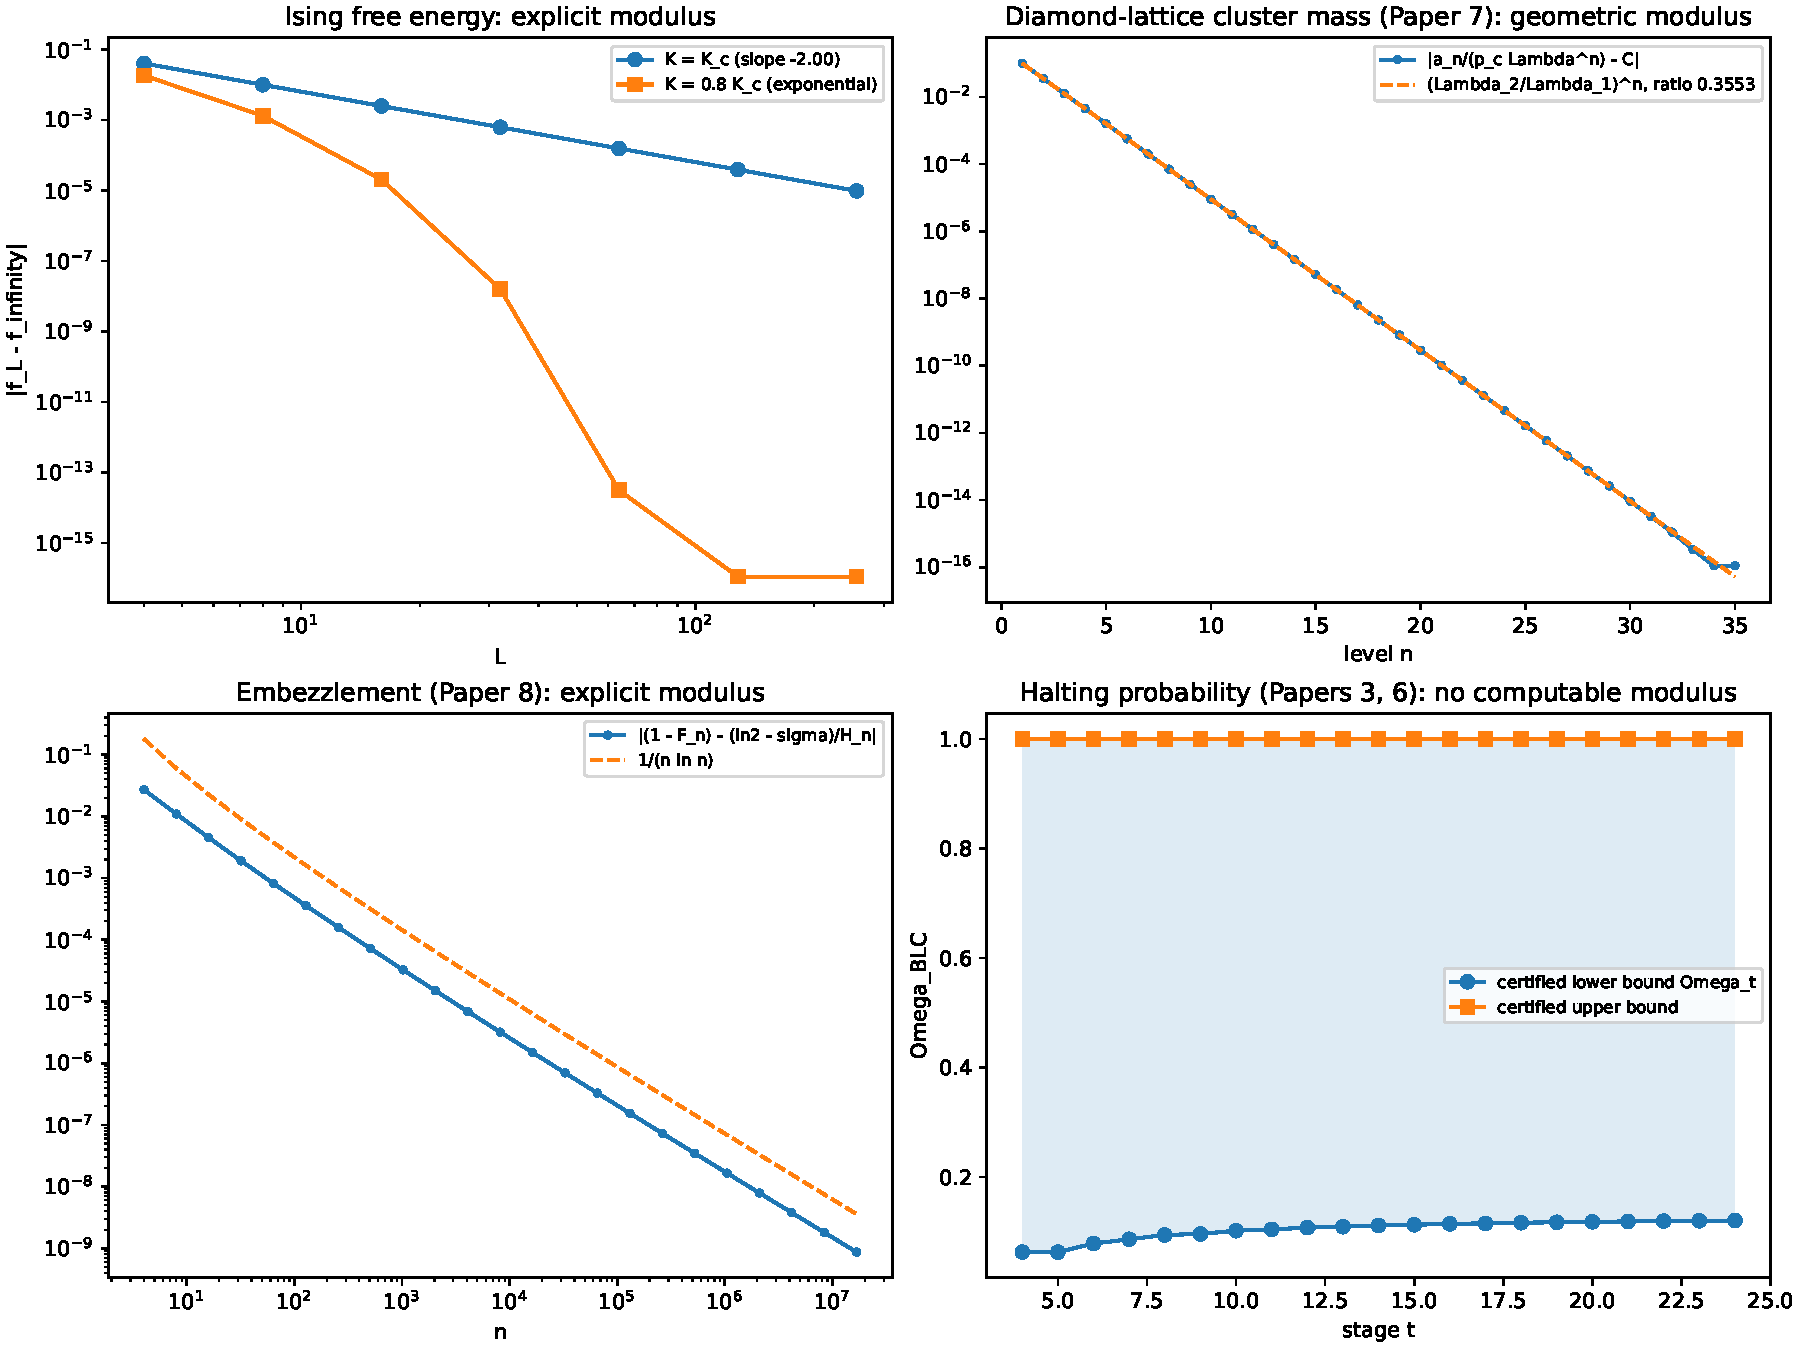
\includegraphics[width=\textwidth]{reverse_math_moduli.pdf}
\caption{Limits with and without computable moduli. \emph{Top left:} error of the exact free energy per site of the
two-dimensional Ising model on an $L\times L$ torus, at $K_c$ ($0.639913/L^2$) and at $0.8K_c$ (exponential). \emph{Top right:}
convergence of the critical-cluster mass of the diamond lattice, with ratio $\Lambda_2/\Lambda_1=0.3553$. \emph{Bottom left:} error of
the embezzlement asymptotics, below $1/(n\ln n)$. \emph{Bottom right:} certified lower and upper bounds for the halting
probability of binary lambda calculus. The lower bound increases, but no computable bound on the remaining distance
exists, and the certified interval does not shrink.}
\label{fig:main}
\end{figure}

%=====================================================================
\section{Background}
\label{sec:background}

We use the standard subsystems of second-order arithmetic~\cite{Simpson}. $\RCA$ consists of basic arithmetic,
$\Sigma^0_1$-induction and $\Delta^0_1$-comprehension; its sets are, informally, those computable from given sets. $\ACA$ adds
comprehension for arithmetical formulas. The collection $\REC$ of all computable sets is an $\omega$-model of $\RCA$ but not
of $\ACA$. A real number is coded by a sequence of rationals $(q_k)$ with $|q_k-q_l|\le2^{-k}$ for $l>k$. In $\REC$ the reals are
exactly the computable reals. $\ACA$ is conservative over $\PA$ for arithmetical sentences~\cite{Simpson}.

We use two facts~\cite[\S\S III.1--III.2]{Simpson}.
\begin{enumerate}
\item[(F1)] Over $\RCA$, $\ACA$ is equivalent to: every bounded nondecreasing sequence of rational numbers converges.
\item[(F2)] Over $\RCA$, $\ACA$ is equivalent to: for every set $X$, the Turing jump $X'$ exists.
\end{enumerate}
The reversal in (F1) goes back to Specker's computable bounded increasing sequence of rationals with a non-computable
limit~\cite{Specker}.

%=====================================================================
\section{Four equivalences}
\label{sec:equivalences}

\subsection{Thermodynamic limits: Fekete's lemma}

The existence of the free energy per site in the thermodynamic limit rests, for translation-invariant interactions, on
subadditivity of $-\ln Z$ and on Fekete's lemma~\cite{Fekete,Ruelle}.

\begin{theorem}
\label{thm:fekete}
Over $\RCA$ the following are equivalent:
\begin{enumerate}
\item[(i)] $\ACA$;
\item[(ii)] for every sequence of reals $(a_n)$ with $a_n\ge0$ and $a_{m+n}\le a_m+a_n$, the limit $\lim_na_n/n$ exists.
\end{enumerate}
\end{theorem}

\begin{proof}
(i)$\Rightarrow$(ii). In $\ACA$ the infimum $\lambda=\inf_na_n/n$ exists, by the least-upper-bound principle for sequences, which
is equivalent to (F1)~\cite{Simpson}. The classical argument then applies. Given $m$, write $n=qm+r$ with $0\le r<m$. Then
$a_n\le qa_m+a_r$, so $a_n/n\le a_m/m+\max_{r<m}a_r/n$, which tends to $a_m/m$. This uses only $\Sigma^0_1$-induction. Hence $\lim
a_n/n=\lambda$.

(ii)$\Rightarrow$(i). Let $(c_n)$ be a nondecreasing sequence of rationals in $[0,1]$, and put $b_n=1-c_n$ and $a_n=nb_n$. Then
$a_n\ge0$, and since $b$ is nonincreasing, $a_{m+n}=(m+n)b_{m+n}\le mb_m+nb_n=a_m+a_n$. By (ii), $a_n/n=b_n$ converges, hence so
does $c_n$, and (F1) gives $\ACA$.
\end{proof}

\begin{remark}
In computability-theoretic terms, Boche, B\"ock and Deppe showed that the Fekete limit of a computable subadditive
sequence is in general not computable, and they classified the associated sets in the arithmetical
hierarchy~\cite{BocheBockDeppe}. Theorem~\ref{thm:fekete} is the corresponding statement in reverse mathematics. For a
specific model the situation can be better. Onsager's solution gives the free energy of the two-dimensional Ising
model as a computable real with explicit finite-size corrections (Section~\ref{sec:instances}).
\end{remark}

\subsection{\texorpdfstring{Infrared limits of $c$-functions}{Infrared limits of c-functions}}

The $c$-theorem asserts that a suitable $c$-function decreases along the renormalisation-group flow, and its infrared
value is the limit~\cite{Zamolodchikov}. The following is a restatement of (F1) in this language.

\begin{corollary}
\label{cor:cfunction}
Over $\RCA$, $\ACA$ is equivalent to: for every bounded nonincreasing sequence $c(r_1)\ge c(r_2)\ge\cdots$ of rationals, indexed
by an increasing sequence of scales, the infrared limit $\lim_kc(r_k)$ exists.
\end{corollary}

For a given flow with an explicit rate of approach to its fixed point, the infrared limit exists already in $\RCA$. The
uniform statement, ``every $c$-function has an infrared value'', has the strength of $\ACA$.

\subsection{Fractal scaling exponents}

In~\cite{Chen2026_chaitin} we considered homogeneous Cantor sets in which every interval at stage $k$ is replaced by its
two end pieces of ratio $r_k=2^{-1/d_k}$, with $d_k=\tfrac14+\tfrac12a_k$. The box-counting and Hausdorff dimensions equal the
scaling exponent
\begin{equation}
D=\lim_{k\to\infty}\frac{k}{\sum_{j\le k}1/d_j}
\label{eq:D}
\end{equation}
whenever it exists. When $a_k$ are lower approximations of Chaitin's $\Omega$, $D=\tfrac14+\tfrac12\Omega$ is not computable.

\begin{theorem}
\label{thm:cantor}
Over $\RCA$ the following are equivalent:
\begin{enumerate}
\item[(i)] $\ACA$;
\item[(ii)] for every nondecreasing sequence $(a_k)$ of rationals in $[0,1)$ the scaling exponent~\eqref{eq:D} exists.
\end{enumerate}
\end{theorem}

\begin{proof}
Put $b_k=1/d_k\in(4/3,4]$, a nonincreasing sequence, and let $\bar b_k=\tfrac1k\sum_{j\le k}b_j$ be its Ces\`aro means. Then~\eqref{eq:D}
states that $1/\bar b_k$ converges.

(i)$\Rightarrow$(ii). By (F1) $b_k$ converges to some $L$. Ces\`aro means of a convergent sequence converge to the same limit,
by an argument that uses only $\Sigma^0_1$-induction, so $D=1/L$.

(ii)$\Rightarrow$(i). Let $\bar b_k\to L$. Since $b$ is nonincreasing, $b_k\le\bar b_k$. For $m>k$,
$\bar b_m\le\bigl(k\bar b_k+(m-k)b_k\bigr)/m$, and letting $m\to\infty$ gives $L\le b_k$. Hence $L\le b_k\le\bar b_k\to L$, so $b_k\to L$. Then
$a_k=2(1/b_k-\tfrac14)$ converges, and (F1) gives $\ACA$.
\end{proof}

\subsection{Connectivity of computable limit sets}

In~\cite{Chen2026_fcu} we constructed computable compact sets $K_e\subset[0,1]^2$ with finite stages $K_{e,n}$, such that the bridge
of $K_e$ is cut at stage $s$ exactly when the $e$-th machine halts at step $s$. Thus $K_e$ is connected if and only if
$K_{e,n}$ is connected for all $n$, if and only if the machine never halts. The construction relativises to an oracle $X$.

\begin{theorem}
\label{thm:connect}
Over $\RCA$ the following are equivalent:
\begin{enumerate}
\item[(i)] $\ACA$;
\item[(ii)] for every set $X$, the set $C^X=\{e:\ K^X_{e,n}\text{ is connected for every }n\}$ exists.
\end{enumerate}
\end{theorem}

\begin{proof}
Each $K^X_{e,n}$ is a finite union of dyadic squares, computable from $X$. By inspection of the construction, $\RCA$ proves
that $K^X_{e,n}$ is disconnected if and only if $n\ge5$ and $\Phi^X_e(e)$ halts within $n$ steps. Hence $e\in C^X$ if and only if $\Phi^X_e(e)$
never halts, so $C^X$ is the complement of $X'$. Thus $C^X$ exists if and only if $X'$ exists, and (F2) gives the equivalence.
\end{proof}

\begin{remark}
We formulated connectivity stage by stage. This avoids formalising the topology of compact sets in second-order
arithmetic, and it is equivalent to connectivity of the limit set by~\cite{Chen2026_fcu}. The same argument applies to the
$\Omega$-comb of~\cite{Chen2026_fcu}. Its attachment pattern computes $\Omega$, and so it does not exist in $\REC$.
\end{remark}

%=====================================================================
\section{Individual limits: computable moduli}
\label{sec:instances}

Equivalences such as Theorems~\ref{thm:fekete}--\ref{thm:connect} concern uniform statements. For a single physical
quantity the relevant question is whether its defining limit has a computable modulus of convergence.

\begin{proposition}
\label{prop:instance}
Let $(x_n)$ be a computable sequence of rationals.
\begin{enumerate}
\item[(a)] If there is a computable $f$ such that $\RCA$ proves $|x_m-x_n|\le2^{-k}$ for all $k$ and all $m,n\ge f(k)$, then $\RCA$ proves
that $\lim_nx_n$ exists.
\item[(b)] If $(x_n)$ converges to a real that is not computable, then $\RCA$ does not prove that $\lim_nx_n$ exists.
\end{enumerate}
\end{proposition}

\begin{proof}
(a) The sequence $(x_{f(k)})_k$ is a code for a real, and $\RCA$ proves that $x_n$ converges to it. (b) $\REC$ is an $\omega$-model of
$\RCA$. In $\REC$ every real is computable, and the statement ``$\lim_nx_n$ exists'' would assert that a computable real equals the
limit, which is false. By soundness, $\RCA$ does not prove the statement.
\end{proof}

We evaluate the moduli of the limits used in the series with the script accompanying this paper.
\begin{itemize}
\item \emph{Ising free energy.} From Kaufman's exact formula on the $L\times L$ torus~\cite{Kaufman} and Onsager's
solution~\cite{Onsager}, the error at $K_c$ is $|f_L-f_\infty|=0.639913/L^2$ at $L=256$. The constant agrees with the universal torus
amplitude of the Ising conformal field theory, $\ln[(\theta_2+\theta_3+\theta_4)/(2\eta)]$ at $\tau=i$, equal to $0.639912$~\cite{DMS}. At
$K=0.8K_c$ the error decays as $e^{-0.490L}$. Both are explicit moduli.
\item \emph{Critical-cluster mass}~\cite{Chen2026_rg}. The mass recursion is linear with matrix entries in $\mathbb Q(\sqrt5)$. The
normalised mass $a_n/(p_c\Lambda^n)$ converges geometrically with ratio $\Lambda_2/\Lambda_1=0.355318$, observed to $10^{-16}$.
\item \emph{Embezzlement}~\cite{Chen2026_certify}. The difference between $1-F_n$ and $(\ln2-\sigma)/H_n$ falls from $2.7\times10^{-2}$ at $n=4$ to
$8.7\times10^{-10}$ at $n=2^{24}$, and $n\ln n$ times it stays below $0.242$.
\item \emph{Halting probability}~\cite{Chen2026_chaitin,Chen2026_fcu}. For binary lambda calculus, the certified lower bound rises
to $0.1202$ at stage $24$, while the certified upper bound stays at $1$. No computable modulus exists for the halting probability of
a universal machine.
\end{itemize}

%=====================================================================
\section{The empirical boundary}
\label{sec:boundary}

Table~\ref{tab:class} collects the limits used in the series, their moduli, and the weakest of the systems considered
here that proves their existence.

\begin{table}[ht]
\centering
\caption{Logical strength of the limits used in the series and their empirical status.}
\label{tab:class}
\small
\begin{tabular}{p{4.6cm}p{3.2cm}p{2.2cm}p{4.2cm}}
\toprule
Limit & Modulus & System & Empirical status \\
\midrule
2D Ising free energy, finite-size error & $0.64/L^2$ at $K_c$, exponential off $K_c$ & $\RCA$ & resolved below experimental precision~\cite{Chen2026_certify} \\
Diamond-lattice cluster mass $d_f=\log_2\Lambda$ & geometric, $0.3553^n$ & $\RCA$ & computed exactly~\cite{Chen2026_rg} \\
Embezzlement fidelity & $O(1/(n\ln n))$ & $\RCA$ & enters explicit certification budget~\cite{Chen2026_certify} \\
Effective dimension of vacuum blocks & finite product bound & $\RCA$ & enters explicit certification budget~\cite{Chen2026_qft} \\
\midrule
Thermodynamic limit, uniform (Fekete) & none in general & $\equiv\ACA$ & --- \\
Infrared limit of $c$-functions, uniform & none in general & $\equiv\ACA$ & --- \\
Cantor scaling exponent, uniform; $D=\tfrac14+\tfrac12\Omega$ & none & $\equiv\ACA$; not $\RCA$ & not certifiable~\cite{Chen2026_chaitin} \\
Connectivity set $C^X$; $\Omega$-comb & none & $\equiv\ACA$; not $\RCA$ & undecidable, no critical scale~\cite{Chen2026_fcu} \\
Finite-dimensional game values $G\mapsto\omega^*(G)$ & none (MIP$^*$=RE) & $\ACA$; not $\RCA$ & bounds not all provable~\cite{Chen2026_certify} \\
\midrule
Resistance exponent $\zeta$ (Lyapunov) & unknown & open & estimated numerically~\cite{Chen2026_rg} \\
Injective $\Leftrightarrow$ semidiscrete (Connes) & --- & open & used in~\cite{Chen2026_qft} \\
\bottomrule
\end{tabular}
\end{table}

For the game values, $\{(G,q):\omega^*(G)>q\}$ is $\Sigma^0_1$, so the function $G\mapsto\omega^*(G)$ exists in $\ACA$. By MIP$^*$=RE~\cite{MIPRE}
it is not computable, so it does not exist in $\REC$.

The table shows the pattern stated in the introduction. Every limit that entered an explicit certification budget has
an explicit modulus and is provable in $\RCA$. Every limit that was shown to be empirically inaccessible is defined
without a computable modulus, and its existence needs $\ACA$. This is not a coincidence. Proposition~\ref{prop:instance}
links logical strength to the existence of a computable modulus. A computable modulus is exactly what a finite procedure
needs in order to know when it has reached a given precision.

%=====================================================================
\section{Discussion}
\label{sec:discussion}

Feferman's thesis is that scientifically applicable mathematics needs only a system conservative over Peano
arithmetic~\cite{Feferman}. Our results refine it for physical limits. The uniform existence theorems for thermodynamic
limits, infrared limits and fractal exponents are equivalent to $\ACA$. This is strictly stronger than $\RCA$, but still
conservative over $\PA$. Individual physical quantities with explicit error bounds need only $\RCA$. The infinite in
physics is therefore real in a precise sense: the general limit theorems cannot be proved from computable set existence
alone. Yet it is logically mild, since it adds no new arithmetical consequences.

Two items remain open. The resistance exponent of the critical diamond-lattice cluster is a Lyapunov exponent of a
random nonlinear recursion. We estimated it numerically, but we have neither a proof that the defining limit exists nor
a closed form or computable modulus, so its logical status is open. The classification of injective von Neumann
algebras, used in~\cite{Chen2026_qft}, rests on deep operator-algebraic machinery whose strength in second-order arithmetic is
unknown.

Together with the earlier papers, the picture is consistent. Physical predictions for finite experiments are computable.
Explicit finite-size and resource bounds are provable from computable set existence. The genuinely infinite content,
including uncomputable dimensions, limit connectivity and the values of infinite-dimensional quantum games, sits exactly
where arithmetical comprehension is needed and where finite experiments cannot reach.

\section*{Data and code availability}
The script \texttt{reverse\_math\_moduli.py}, the data (CSV), the figure and the console output are available at
\url{https://github.com/Ruqing1963/reverse-math-physics} and archived under DOI \href{https://doi.org/\paperdoi}{\paperdoi}.

%=====================================================================
\begin{thebibliography}{99}\small
\bibitem{Friedman} H.~Friedman, ``Some systems of second order arithmetic and their use'', in \emph{Proceedings of the International Congress of Mathematicians (Vancouver, 1974)}, Vol.~1, Canadian Mathematical Congress (1975) 235--242.
\bibitem{Simpson} S.~G.~Simpson, \emph{Subsystems of Second Order Arithmetic}, 2nd ed., Perspectives in Logic, Cambridge University Press and Association for Symbolic Logic (2009).
\bibitem{Feferman} S.~Feferman, ``Why a little bit goes a long way: Logical foundations of scientifically applicable mathematics'', in \emph{PSA 1992}, Vol.~2, Philosophy of Science Association (1993) 442--455.
\bibitem{Chen2026_chaitin} R.~Chen, ``Uncomputable fractal dimensions, Kolmogorov complexity cascades, and the Chaitin barrier in physical systems'' (2026), doi:10.5281/zenodo.23194419.
\bibitem{Chen2026_fcu} R.~Chen, ``Undecidable connectivity of computable fractal limit sets: $\Pi^0_1$-completeness, an $\Omega$-comb, and incompleteness thresholds'' (2026), doi:10.5281/zenodo.23199984.
\bibitem{Chen2026_certify} R.~Chen, ``Can finite experiments certify actual infinity? Dimension witnesses, Tsirelson's problem, and holographic resource bounds'' (2026), doi:10.5281/zenodo.23202129.
\bibitem{Chen2026_qft} R.~Chen, ``Closing the Tsirelson loophole in relativistic quantum field theory: Split inclusions, hyperfinite local algebras, and the effective dimension of the vacuum'' (2026), doi:10.5281/zenodo.23202937.
\bibitem{Chen2026_rg} R.~Chen, ``Renormalization group flows of spectral dimensions on hierarchical lattices: Critical percolation, resistance exponents, and transport universality'' (2026), doi:10.5281/zenodo.23201028.
\bibitem{Specker} E.~Specker, ``Nicht konstruktiv beweisbare S\"atze der Analysis'', J.\ Symbolic Logic 14 (1949) 145--158.
\bibitem{Fekete} M.~Fekete, ``\"Uber die Verteilung der Wurzeln bei gewissen algebraischen Gleichungen mit ganzzahligen Koeffizienten'', Math.\ Z.\ 17 (1923) 228--249.
\bibitem{Ruelle} D.~Ruelle, \emph{Statistical Mechanics: Rigorous Results}, Benjamin, New York (1969).
\bibitem{BocheBockDeppe} H.~Boche, Y.~B\"ock, C.~Deppe, ``On effective convergence in Fekete's lemma and related combinatorial problems in information theory'', arXiv:2010.09896.
\bibitem{Zamolodchikov} A.~B.~Zamolodchikov, ``Irreversibility of the flux of the renormalization group in a 2D field theory'', JETP Lett.\ 43 (1986) 730--732.
\bibitem{Kaufman} B.~Kaufman, ``Crystal statistics. II. Partition function evaluated by spinor analysis'', Phys.\ Rev.\ 76 (1949) 1232--1243.
\bibitem{Onsager} L.~Onsager, ``Crystal statistics. I. A two-dimensional model with an order-disorder transition'', Phys.\ Rev.\ 65 (1944) 117--149.
\bibitem{DMS} P.~Di Francesco, P.~Mathieu, D.~S\'en\'echal, \emph{Conformal Field Theory}, Springer, New York (1997).
\bibitem{MIPRE} Z.~Ji, A.~Natarajan, T.~Vidick, J.~Wright, H.~Yuen, ``MIP$^*$=RE'', arXiv:2001.04383 (2020).
\end{thebibliography}

\end{document}
